\documentclass{article}
\usepackage[utf8]{inputenc}
\usepackage{amsmath}
\usepackage{tikz}

\title{Master 2 CSMI : EDP2\\Rapport de TP}
\author{Romain Vallet}

\begin{document}

\maketitle

\section{TP 1}

Les codes de la résolution numérique du schéma de Godunov est placé dans un repository sous github ($https://github.com/ValletRomain/edp_tp1$).

\subsection{Résolution numérique de l’équation de transport}

1.

\[ \left\{ \begin{matrix}
\partial_t u + c \partial_x u &=& 0 \text{ avec } t \in ]0,T[ \text{ et } x \in ]0,L[  \\
u(0,t) &=& e^{-t} \text{ avec } t \in ]0,T[ \\
u(x,0) &=& 0 \text{ avec } x \in ]0,L[
\end{matrix} \right.
\label{trans1} \tag{Transport1} \]

Avec $c>0$
\newline

La solution de \ref{trans1} est de la forme :

\[
\left\{
\begin{array}{ll}
    u(x,t) = u(x-ct,0) = 0 \text{ avec } x \geq ct \\
    u(x,t) = u(0,t-\frac{x}{c}) = e^{\frac{x}{c}-t} \text{ avec } x < ct
\end{array}
\right.
\tag{Sol1}
\]

2. Si $c < 0$ :

On a pour $t \in ]0,T[$, $-ct>0$, avec l'analyse des courbes caractéristiques, nous avons :

\begin{eqnarray*}
u(0,t) &=& u(-ct,0) \\
e^{-t} &=& 0
\end{eqnarray*}

Nous avons une contradiction, il n'y a pas de solution.
\newline

3.

4.

5.

\subsection{Résolution numérique de l’équation de Burgers}

1. 

\[ \left\{ \begin{matrix}
	\partial_t u + \partial_x(\frac{u^2}{2}) &=& 0 \textbf{, } x \in ]-1,2[ \\
	u(0,t) &=& 1, \\
	u(x,0) &=& \left\{ \begin{matrix}
		1 \text{ si } x<0 \\
		1-x \text{ si } 0\leq x \leq 1 \\
		0 \text{ si } x>1	
	\end{matrix} \right.
\end{matrix} \right.
\label{eq3} \tag{Burgers1}
\]

On va utiliser la méthode de la caractéristique. On cherche $t \longmapsto x(t)$ tel que $u(x(t),t) = cte$.

On suppose qu'il existe un tel $x(t)$, d'une part, on a :

\begin{eqnarray*}
	\frac{\partial (u(x(t),t))}{\partial t} &=& 0 \\
	\frac{\partial u}{\partial t}(x(t),t) + x'(t) \frac{\partial u}{\partial x}(x(t),t) &=& 0
\end{eqnarray*}

D'autre part $u$ vérifie l'équation du burgers :

\begin{eqnarray*}
	\frac{\partial u}{\partial t} + \frac{\partial (u^2/2)}{\partial x} = 0 \\
	\frac{\partial u}{\partial t} + u \frac{\partial u}{\partial x} = 0 \\
	\frac{\partial u}{\partial t}(x(t),t) + u(x(t),t) \frac{\partial u}{\partial x}(x(t),t) = 0 
\end{eqnarray*}

Par identification, on a :
\[ x'(t) = u(x(t),t) \]

Et puisque $t \longmapsto x(t)$ est une courbe caractéristique, on a :
\[x'(t) = u(x(0),0) = cte\]

Donc $t \longmapsto x(t)$ est une droite.

Si une courbe caractéristique existe alors c'est une droite de direction $u(x(0),0)$.
\newline

Remarque : $u(x,t) = u(x_0,0)$ avec $x_0$ tel que $x = u(x_0,0) t + x_0$.
\newline

Réciproquement, prenons une tel courbe et prouvons quelle est caractéristique. Soit $x_0 \in R$ et $t \longmapsto x(t) = u(x_0,0) t + x_0$ :

\begin{eqnarray*}
	\frac{d (u(x(t),t))}{dt} &=& x'(t) \frac{\partial u}{\partial x}(x(t),t) + \frac{\partial u}{\partial t}(x(t),t) \\
	&=& u(x(0),0) \frac{\partial u}{\partial x}(x(t),t) + \frac{\partial u}{\partial t}(x(t),t) \\
	&=& u(x(0),0) \frac{\partial u}{\partial x}(x(t),t) - u(x(t),t) \frac{\partial u}{\partial x}(x(t),t) \\
	&=& \frac{\partial u}{\partial x}(x(t),t) \left( u(x(0),0)-u(x(t),t) \right) \\
	&=& 
\end{eqnarray*}

Alors, les courbes caractéristiques sont de la forme $t longmapsto x(t) = u(x_0,0) t + x_0$.

On a alors :

\[
x(t) = \left\{ \begin{matrix}
	t + x_0 \text{ pour } x_0 < 0 \\
	(1-x_0) t + x_0 \text{ pour } 0 \leq x_0 \leq 1 \\
	x_0 \text{ pour } x_0 > 1
\end{matrix} \right. \]

\begin{figure}
  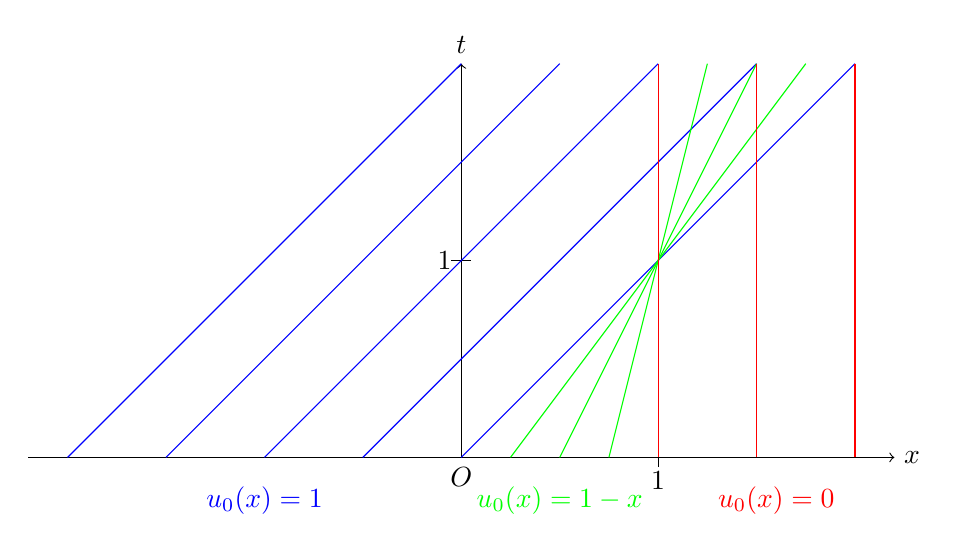
\begin{tikzpicture}[scale=2.5]
\draw[->] (-2.2,0) -- (2.2,0);
\draw (2.2,0) node[right] {$x$};
\draw[->] (0,0) -- (0,2);
\draw (0,2) node[above] {$t$};
\draw (0,0) node[below] {$O$};
\draw (1,-0.05) -- (1,0.05);
\draw (1,-0.025) node[below] {$1$};
\draw (-0.05,1) -- (0.05,1);
\draw (0,1) node[left] {$1$};

\draw[blue] (-2,0) -- (0,2);
\draw[blue] (-1.5,0) -- (0.5,2);
\draw[blue] (-1,0) -- (1,2);
\draw[blue] (-0.5,0) -- (1.5,2);
\draw[blue] (0,0) -- (2,2);
\draw[blue] (-1,-0.1) node[below] {$u_0(x)=1$};

\draw[green] (0.25,0) -- (1.75,2);
\draw[green] (0.5,0) -- (1.5,2);
\draw[green] (0.75,0) -- (1.25,2);
\draw[green] (0.5,-0.1) node[below] {$u_0(x)=1-x$};

\draw[red] (1,0) -- (1,2);
\draw[red] (1.5,0) -- (1.5,2);
\draw[red] (2,0) -- (2,2);
\draw[red] (1.6,-0.1) node[below] {$u_0(x)=0$};
\end{tikzpicture}
  \caption{Courbes caractéristiques \ref{eq3}}
\end{figure}

On voit que deux courbes peuvent se croiser. Nous obtenons 4 zones.

\begin{figure} 
  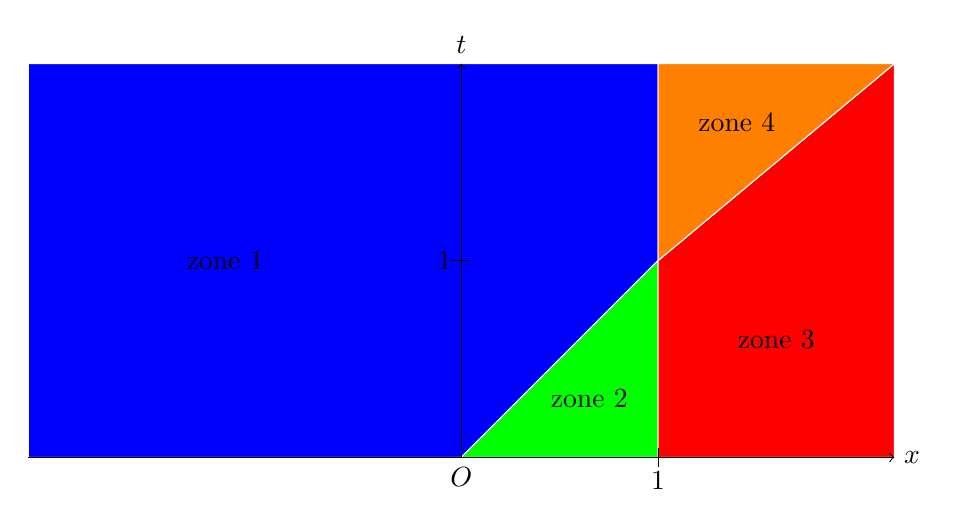
\begin{tikzpicture}[scale=2.5]
\draw[color=white, fill=blue] (-2.2,0) -- (0,0) -- (1,1) -- (1,2) -- (-2.2,2) -- cycle;
\draw (-1.2,1) node {zone 1};

\draw[color=white, fill=green] (0,0) -- (1,0) -- (1,1) -- cycle;
\draw (0.65,0.3) node {zone 2};

\draw[color=white, fill=red] (1,0) -- (2.2,0) -- (2.2,2) -- (1,1) -- cycle;
\draw (1.6,0.6) node {zone 3};

\draw[color=white, fill=orange] (1,1) -- (2.2,2) -- (1,2) -- cycle;
\draw (1.4,1.7) node {zone 4};

\draw[->] (-2.2,0) -- (2.2,0);
\draw (2.2,0) node[right] {$x$};
\draw[->] (0,0) -- (0,2);
\draw (0,2) node[above] {$t$};
\draw (0,0) node[below] {$O$};
\draw (1,-0.05) -- (1,0.05);
\draw (1,-0.025) node[below] {$1$};
\draw (-0.05,1) -- (0.05,1);
\draw (0,1) node[left] {$1$};
\end{tikzpicture}
  \caption{Différentes zones \ref{eq3}}
\end{figure}

La zone 1 ($\{(x,t) \in R \times R^{+}, x < 1, t > x\}$) donne $u(x,t) = 1$.

La zone 2 ($\{(x,t) \in R \times R^{+}, x > 1, t < x\}$) donne $u(x,t) = 0$.

La zone 3 ($\{(x,t) \in R \times R^{+}, 0 < x < 1, x < t \}$), nous donne :

\begin{eqnarray*}
	u(x,t) &=& 1 - x_0 \text{ avec } x = (1-x_0) t + x_0 \\
	u(x,t) &=& 1 - \frac{x-t}{1-t} \text{ en effet } x_0 = \frac{x-t}{1-t} \\
	u(x,t) &=& \frac{1-x}{1-t}  
\end{eqnarray*}

La zone 4 ($\{(x,t) \in R \times R^+, x > 1, t > x\}$), nous donne :

Pour trouver la valeur de $u(x,t)$, nous devons intégrer un choc. Nous avons $u_L=1$ et $u_R=0$. Donc la vitesse du choc s'exprime :
\[ \frac{dx}{dt} = \sigma = \frac{u_L^2/2 - u_R^2/2}{u_L - u_R} = \frac{1}{2} \frac{(u_L-u_R)(u_L+u_R)}{u_L-u_R} = \frac{u_L+u_R}{2} = \frac{1}{2} \]

Donc le choc se trouve sur la droite de pente $2$ et passant par $(1,1)$ :
\[ x = 2 (t - 1) + 1 = 2t + 2 \]

On obtiens que sur $\text{zone 4 } \cap \{(x,t), t+1 > x/2\}$, $u(x,t) = 1$ et sur $\text{zone 4 } \cap \{(x,t), t+1 < x/2\}$, $u(x,t) = 0$.
\newline

Nous avons résolue le problème au sens de Lax et la solution est : 

\[u(x,t) = \left\{ \begin{matrix}
	1 \text{ pour } x<1, t>x \text{ ou } x>1, t+1>x/2 \\
	\frac{1-x}{1-t} \text{ pour } 0<x<1 \text{ ou } x<t \\
	0 \text{ pour } x>1, t+1<x/2
\end{matrix} \right.
\tag{Sol3}
\]

\begin{figure}
  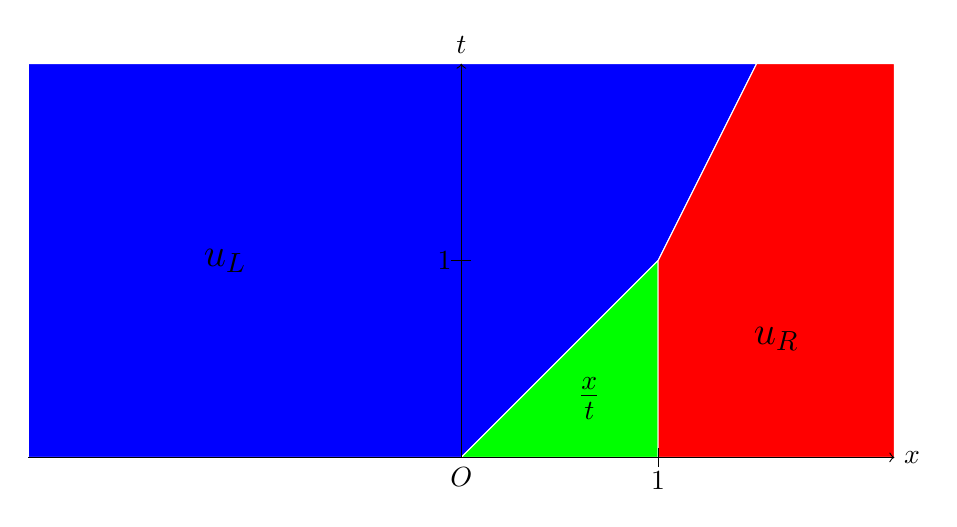
\begin{tikzpicture}[scale=2.5]
\draw[color=white, fill=blue] (-2.2,0) -- (0,0) -- (1,1) -- (1.5,2) -- (-2.2,2) -- cycle;
\draw (-1.2,1) node {\Large{$u_L$}};

\draw[color=white, fill=green] (0,0) -- (1,0) -- (1,1) -- cycle;
\draw (0.65,0.3) node {\Large{$\frac{x}{t}$}};

\draw[color=white, fill=red] (1,0) -- (2.2,0) -- (2.2,2) -- (1.5,2) -- (1,1) -- cycle;
\draw (1.6,0.6) node {\Large{$u_R$}};

\draw[->] (-2.2,0) -- (2.2,0);
\draw (2.2,0) node[right] {$x$};
\draw[->] (0,0) -- (0,2);
\draw (0,2) node[above] {$t$};
\draw (0,0) node[below] {$O$};
\draw (1,-0.05) -- (1,0.05);
\draw (1,-0.025) node[below] {$1$};
\draw (-0.05,1) -- (0.05,1);
\draw (0,1) node[left] {$1$};
\end{tikzpicture}
  \caption{Solution de l'équation \ref{eq3}}
\end{figure}

2. Résolvons le problème de Riemann pour l'équation de Burgers :

\[ \left\{ \begin{matrix}
	\frac{\partial u}{\partial t} + \frac{\partial (u^2/2)}{\partial x} = 0 \\
	u(x,0) = \left\{ \begin{matrix}
					u_L \text{ pour } x<0 \\
					u_R \text{ pour } x>0
	\end{matrix} \right.
\end{matrix} \right.
\label{eq4} \tag{Burgers2}
\]

Nous avons vu précédement que les courbes caractéristiques de l'équation de Burgers sont des droites de pente $u(x_0,0)^{-1}$. Soit pour $x_0<0$, ces droites ont une pente de $u_L^{-1}$ et pour $x_0>0$, elles ont une pente $u_R^{-1}$.
\newline

Nous avons deux cas :

$\bullet$ $u_L < u_R$, alors $u_L^{-1} > u_R^{-1}$. Les courbes caractéristiques ne se rencontrent pas.

\begin{figure}
  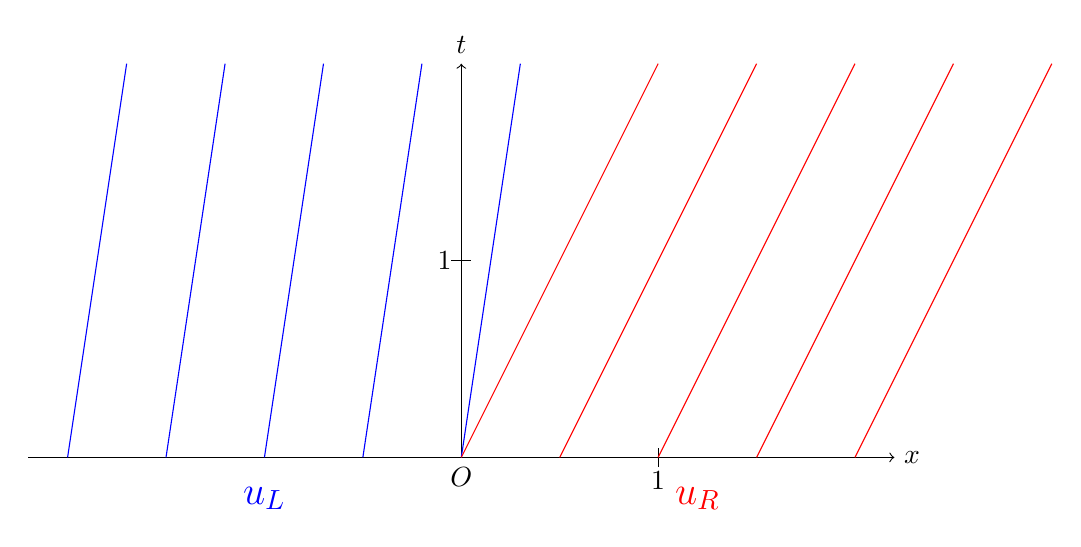
\begin{tikzpicture}[scale=2.5]
\draw[->] (-2.2,0) -- (2.2,0);
\draw (2.2,0) node[right] {$x$};
\draw[->] (0,0) -- (0,2);
\draw (0,2) node[above] {$t$};
\draw (0,0) node[below] {$O$};
\draw (1,-0.05) -- (1,0.05);
\draw (1,-0.025) node[below] {$1$};
\draw (-0.05,1) -- (0.05,1);
\draw (0,1) node[left] {$1$};

\draw[blue] (-2,0) -- (-1.7,2);
\draw[blue] (-1.5,0) -- (-1.2,2);
\draw[blue] (-1,0) -- (-0.7,2);
\draw[blue] (-0.5,0) -- (-0.2,2);
\draw[blue] (0,0) -- (0.3,2);
\draw[blue] (-1,-0.1) node[below] {\Large{$u_L$}};

\draw[red] (0,0) -- (1,2);
\draw[red] (0.5,0) -- (1.5,2);
\draw[red] (1,0) -- (2,2);
\draw[red] (1.5,0) -- (2.5,2);
\draw[red] (2,0) -- (3,2);
\draw[red] (1.2,-0.1) node[below] {\Large{$u_R$}};
\end{tikzpicture}
  \caption{Courbes caractéristiques pour $u_L < u_R$ \ref{eq4}}
\end{figure}

Nous avons trois zones :

- $zone1 = (x,t)$ tel que $x < u_L t$, on a $u(x,t) = u_L$

- $zone2 = (x,t)$ tel que $x > u_R t$, on a $u(x,t) = u_R$

- $zone3 = (x,t)$ tel que $u_L t < x < u_R t$ qui est plus complexe.

\begin{figure}
  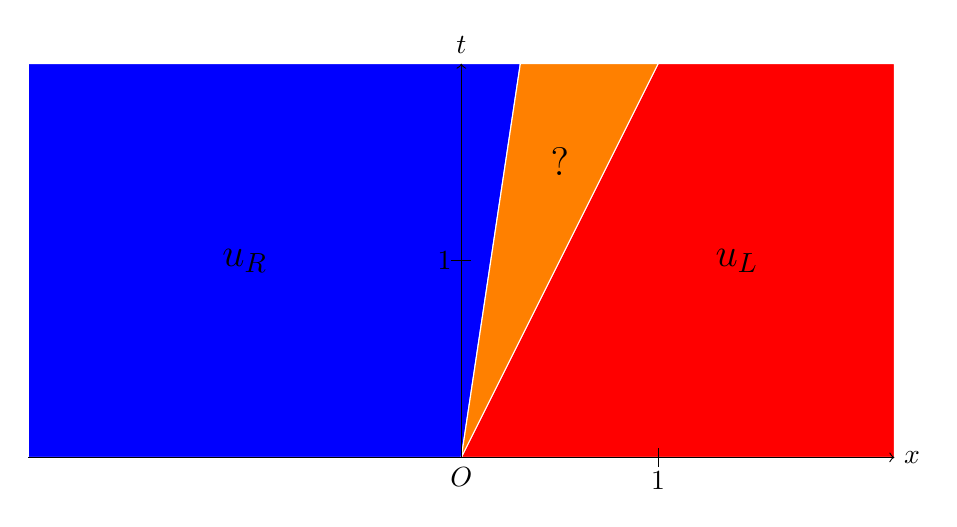
\begin{tikzpicture}[scale=2.5]
\draw[color=white, fill=blue] (-2.2,0) -- (0,0) -- (0.3,2) -- (-2.2,2) -- cycle;
\draw (-1.1,1) node {\Large{$u_R$}};

\draw[color=white, fill=red] (0,0) -- (2.2,0) -- (2.2,2) -- (1,2) -- cycle;
\draw (1.4,1) node {\Large{$u_L$}};

\draw[color=white, fill=orange] (0,0) -- (1,2) -- (0.3,2) -- cycle;
\draw (0.5,1.5) node {\Large{?}};

\draw[->] (-2.2,0) -- (2.2,0);
\draw (2.2,0) node[right] {$x$};
\draw[->] (0,0) -- (0,2);
\draw (0,2) node[above] {$t$};
\draw (0,0) node[below] {$O$};
\draw (1,-0.05) -- (1,0.05);
\draw (1,-0.025) node[below] {$1$};
\draw (-0.05,1) -- (0.05,1);
\draw (0,1) node[left] {$1$};
\end{tikzpicture}
  \caption{Différentes zones $u_L < u_R$ \ref{eq4}}
\end{figure}

Résolvons l'équation sur la deuxième partie. On veut trouver une fonction sur cet ensemble qui vérifie l'équation de Burgers et que la fonction globale soit continue.

Regardons $u(x,t) = \frac{x}{t}$ sur $zone1$. Ce raccord fonctionne-t'il ?

D'une part :
\[ \frac{\partial f}{\partial t}(x,t) = -\frac{x}{t^2} \]


D'autre part :
\[ f(x,t) \frac{\partial f}{\partial}(x,t) = \frac{x}{t} \times \frac{1}{t} = \frac{x}{t^2} \]

On a que $f$ vérifie l'équation de Burgers sur la $zone3$.
\[ \frac{\partial f}{\partial t}(x,t) + f(x,t) \frac{\partial f}{\partial}(x,t) = -\frac{x}{t^2} + \frac{x}{t^2} = 0 \]

Maintenant, regardons si la fonction globale  (qui vérifie l'équation)
\[
u(x,t) = \left\{ \begin{matrix}
			u_L \text{ pour } x < u_L t \\
			f(x,t) \text{ pour } u_L t < x < u_R t \\
			u_R \text{ pour } x > u_R t
\end{matrix} \right.
\tag{Sol4.1}
\]

est continue.

$f$ est continue sur les 3 zones, il faut regarder aux frontières :

Pour $x = u_L t$ : $f(x,t) = \frac{u_L t}{t} = u_L$ et pour $x = u_R t$ : $f(x,t) = \frac{u_R t}{t} = u_R$.
\newline

Alors la fonction $u$ vérifie l'équation au sens de Lax.

\begin{figure}
  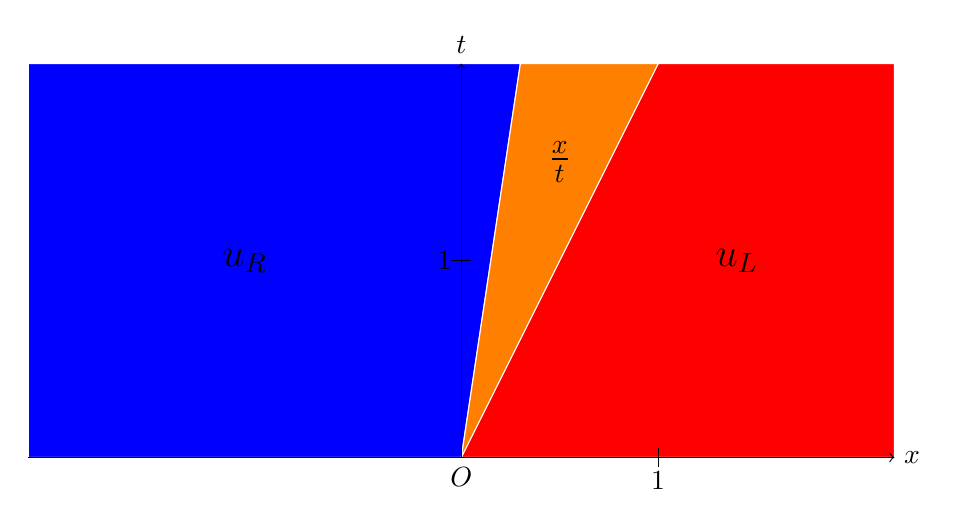
\begin{tikzpicture}[scale=2.5]
\draw[color=white, fill=blue] (-2.2,0) -- (0,0) -- (0.3,2) -- (-2.2,2) -- cycle;
\draw (-1.1,1) node {\Large{$u_R$}};

\draw[color=white, fill=red] (0,0) -- (2.2,0) -- (2.2,2) -- (1,2) -- cycle;
\draw (1.4,1) node {\Large{$u_L$}};

\draw[color=white, fill=orange] (0,0) -- (1,2) -- (0.3,2) -- cycle;
\draw (0.5,1.5) node {\Large{$\frac{x}{t}$}};

\draw[->] (-2.2,0) -- (2.2,0);
\draw (2.2,0) node[right] {$x$};
\draw[->] (0,0) -- (0,2);
\draw (0,2) node[above] {$t$};
\draw (0,0) node[below] {$O$};
\draw (1,-0.05) -- (1,0.05);
\draw (1,-0.025) node[below] {$1$};
\draw (-0.05,1) -- (0.05,1);
\draw (0,1) node[left] {$1$};
\end{tikzpicture}
  \caption{Solution de l'équation $u_L < u_R$ \ref{eq4}}
\end{figure}


$\bullet$ $u_L > u_R$, alors $u_L^{-1} < u_R^{-1}$. Les courbes caractéristiques se rencontrent (toutes les courbes de droite rencontre toutes les courbes de gauche).

\begin{figure}
  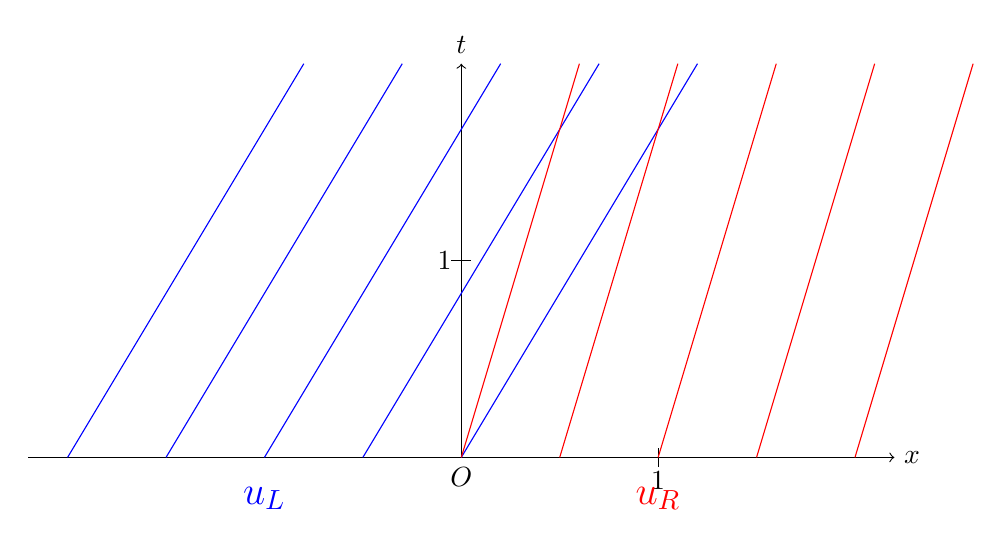
\begin{tikzpicture}[scale=2.5]
\draw[->] (-2.2,0) -- (2.2,0);
\draw (2.2,0) node[right] {$x$};
\draw[->] (0,0) -- (0,2);
\draw (0,2) node[above] {$t$};
\draw (0,0) node[below] {$O$};
\draw (1,-0.05) -- (1,0.05);
\draw (1,-0.025) node[below] {$1$};
\draw (-0.05,1) -- (0.05,1);
\draw (0,1) node[left] {$1$};

\draw[blue] (-2,0) -- (-0.8,2);
\draw[blue] (-1.5,0) -- (-0.3,2);
\draw[blue] (-1,0) -- (0.2,2);
\draw[blue] (-0.5,0) -- (0.7,2);
\draw[blue] (0,0) -- (1.2,2);
\draw[blue] (-1,-0.1) node[below] {\Large{$u_L$}};

\draw[red] (0,0) -- (0.6,2);
\draw[red] (0.5,0) -- (1.1,2);
\draw[red] (1,0) -- (1.6,2);
\draw[red] (1.5,0) -- (2.1,2);
\draw[red] (2,0) -- (2.6,2);
\draw[red] (1,-0.1) node[below] {\Large{$u_R$}};
\end{tikzpicture}
  \caption{Courbes caractéristiques $u_L > u_R$ \ref{eq4}}
\end{figure}

Il faut intégrer un choc de vitesse $\sigma$, comme calculer dans la question précédente, nous avons :
\[ \sigma = \frac{u_L+u_R}{2} \]

La frontière du choc est une droite de pente $\sigma^{-1}$ et d'origine $(0,0)$. Soit une droite d'équation : $x = \sigma t$. Une solution au sens de Lax est :

\[ u(x,t) = \left\{ \begin{matrix}
				u_L \text{ pour } x < \sigma t \\
				u_R \text{ pour } x > \sigma t \\
\end{matrix}\right.
\tag{Sol4.2} \]

\begin{figure}
  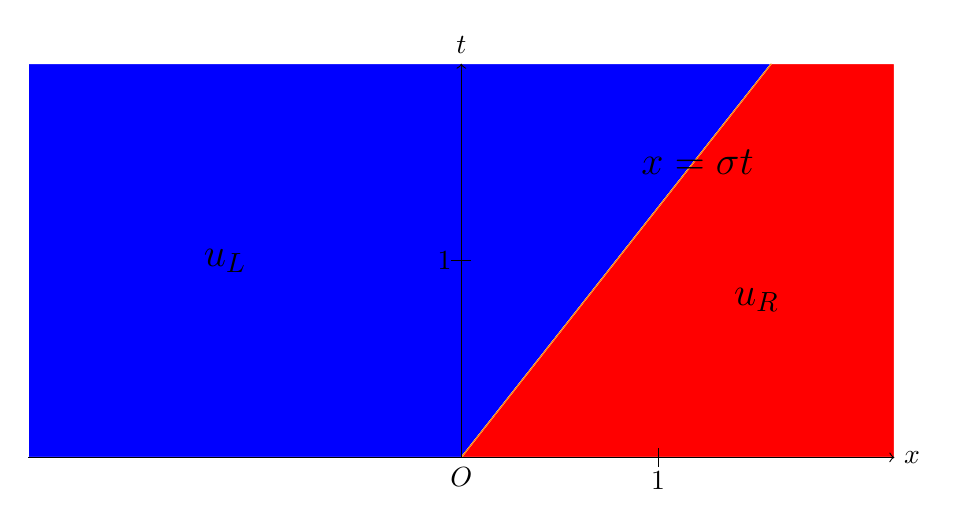
\begin{tikzpicture}[scale=2.5]
\draw[color=white, fill=blue] (-2.2,0) -- (0,0) -- (1.575,2) -- (-2.2,2) -- cycle;
\draw (-1.2,1) node {\Large{$u_L$}};
\draw[color=white, fill=red] (0,0) -- (2.2,0) -- (2.2,2) -- (1.575,2) -- cycle;
\draw (1.5,0.8) node {\Large{$u_R$}};
\draw[color=orange] (0,0) -- (1.575,2);
\draw (1.2,1.5) node{\Large{$x = \sigma t$}};

\draw[->] (-2.2,0) -- (2.2,0);
\draw (2.2,0) node[right] {$x$};
\draw[->] (0,0) -- (0,2);
\draw (0,2) node[above] {$t$};
\draw (0,0) node[below] {$O$};
\draw (1,-0.05) -- (1,0.05);
\draw (1,-0.025) node[below] {$1$};
\draw (-0.05,1) -- (0.05,1);
\draw (0,1) node[left] {$1$};
\end{tikzpicture}
  \caption{Solution de l'équation $u_L > u_R$ \ref{eq4}}
\end{figure}

3.

4.

\section{TP2}

\subsection{Résolution numérique du système de Saint-Venant}

1.

2.

3.

4.

5.

6.

7.

8.

9.

10.

11.

\section{TP3}

\subsection{Résolution numérique du système de Saint-Venant en deux dimensions}

1.

2.

3.

4.

5.

6.

7.

8.

\end{document}
